\documentclass[twoside]{book}

% Packages required by doxygen
\usepackage{calc}
\usepackage{doxygen}
\usepackage{graphicx}
\usepackage[utf8]{inputenc}
\usepackage{makeidx}
\usepackage{multicol}
\usepackage{multirow}
\PassOptionsToPackage{warn}{textcomp}
\usepackage{textcomp}
\usepackage[nointegrals]{wasysym}
\usepackage[table]{xcolor}

% Font selection
\usepackage[T1]{fontenc}
\usepackage{mathptmx}
\usepackage[scaled=.90]{helvet}
\usepackage{courier}
\usepackage{amssymb}
\usepackage{sectsty}
\renewcommand{\familydefault}{\sfdefault}
\allsectionsfont{%
  \fontseries{bc}\selectfont%
  \color{darkgray}%
}
\renewcommand{\DoxyLabelFont}{%
  \fontseries{bc}\selectfont%
  \color{darkgray}%
}
\newcommand{\+}{\discretionary{\mbox{\scriptsize$\hookleftarrow$}}{}{}}

% Page & text layout
\usepackage{geometry}
\geometry{%
  letterpaper,%
  top=2.5cm,%
  bottom=2.5cm,%
  left=2.5cm,%
  right=2.5cm%
}
\tolerance=750
\hfuzz=15pt
\hbadness=750
\setlength{\emergencystretch}{15pt}
\setlength{\parindent}{0cm}
\setlength{\parskip}{0.2cm}
\makeatletter
\renewcommand{\paragraph}{%
  \@startsection{paragraph}{4}{0ex}{-1.0ex}{1.0ex}{%
    \normalfont\normalsize\bfseries\SS@parafont%
  }%
}
\renewcommand{\subparagraph}{%
  \@startsection{subparagraph}{5}{0ex}{-1.0ex}{1.0ex}{%
    \normalfont\normalsize\bfseries\SS@subparafont%
  }%
}
\makeatother

% Headers & footers
\usepackage{fancyhdr}
\pagestyle{fancyplain}
\fancyhead[LE]{\fancyplain{}{\bfseries\thepage}}
\fancyhead[CE]{\fancyplain{}{}}
\fancyhead[RE]{\fancyplain{}{\bfseries\leftmark}}
\fancyhead[LO]{\fancyplain{}{\bfseries\rightmark}}
\fancyhead[CO]{\fancyplain{}{}}
\fancyhead[RO]{\fancyplain{}{\bfseries\thepage}}
\fancyfoot[LE]{\fancyplain{}{}}
\fancyfoot[CE]{\fancyplain{}{}}
\fancyfoot[RE]{\fancyplain{}{\bfseries\scriptsize Generated on Wed Apr 9 2014 20\+:35\+:35 for M\+E405 Lab 1 -\/ A\+D\+C by Doxygen }}
\fancyfoot[LO]{\fancyplain{}{\bfseries\scriptsize Generated on Wed Apr 9 2014 20\+:35\+:35 for M\+E405 Lab 1 -\/ A\+D\+C by Doxygen }}
\fancyfoot[CO]{\fancyplain{}{}}
\fancyfoot[RO]{\fancyplain{}{}}
\renewcommand{\footrulewidth}{0.4pt}
\renewcommand{\chaptermark}[1]{%
  \markboth{#1}{}%
}
\renewcommand{\sectionmark}[1]{%
  \markright{\thesection\ #1}%
}

% Indices & bibliography
\usepackage{natbib}
\usepackage[titles]{tocloft}
\setcounter{tocdepth}{3}
\setcounter{secnumdepth}{5}
\makeindex

% Hyperlinks (required, but should be loaded last)
\usepackage{ifpdf}
\ifpdf
  \usepackage[pdftex,pagebackref=true]{hyperref}
\else
  \usepackage[ps2pdf,pagebackref=true]{hyperref}
\fi
\hypersetup{%
  colorlinks=true,%
  linkcolor=blue,%
  citecolor=blue,%
  unicode%
}

% Custom commands
\newcommand{\clearemptydoublepage}{%
  \newpage{\pagestyle{empty}\cleardoublepage}%
}


%===== C O N T E N T S =====

\begin{document}

% Titlepage & ToC
\hypersetup{pageanchor=false,
             bookmarks=true,
             bookmarksnumbered=true,
             pdfencoding=unicode
            }
\pagenumbering{roman}
\begin{titlepage}
\vspace*{7cm}
\begin{center}%
{\Large M\+E405 Lab 1 -\/ A\+D\+C \\[1ex]\large 1.\+0 }\\
\vspace*{1cm}
{\large Generated by Doxygen 1.8.6}\\
\vspace*{0.5cm}
{\small Wed Apr 9 2014 20:35:35}\\
\end{center}
\end{titlepage}
\clearemptydoublepage
\tableofcontents
\clearemptydoublepage
\pagenumbering{arabic}
\hypersetup{pageanchor=true}

%--- Begin generated contents ---
\chapter{Hierarchical Index}
\section{Class Hierarchy}
This inheritance list is sorted roughly, but not completely, alphabetically\+:\begin{DoxyCompactList}
\item \contentsline{section}{adc}{\pageref{classadc}}{}
\item frt\+\_\+task\begin{DoxyCompactList}
\item \contentsline{section}{task\+\_\+brightness}{\pageref{classtask__brightness}}{}
\item \contentsline{section}{task\+\_\+user}{\pageref{classtask__user}}{}
\end{DoxyCompactList}
\end{DoxyCompactList}

\chapter{Class Index}
\section{Class List}
Here are the classes, structs, unions and interfaces with brief descriptions\+:\begin{DoxyCompactList}
\item\contentsline{section}{\hyperlink{classadc}{adc} \\*This class should run the A/\+D converter on an A\+V\+R processor }{\pageref{classadc}}{}
\item\contentsline{section}{\hyperlink{classtask__brightness}{task\+\_\+brightness} \\*This task controls the brightness of an L\+E\+D using an analog input from the A/\+D converter }{\pageref{classtask__brightness}}{}
\item\contentsline{section}{\hyperlink{classtask__user}{task\+\_\+user} }{\pageref{classtask__user}}{}
\end{DoxyCompactList}

\chapter{File Index}
\section{File List}
Here is a list of all documented files with brief descriptions\+:\begin{DoxyCompactList}
\item\contentsline{section}{\hyperlink{adc_8cpp}{adc.\+cpp} }{\pageref{adc_8cpp}}{}
\item\contentsline{section}{\hyperlink{adc_8h}{adc.\+h} }{\pageref{adc_8h}}{}
\item\contentsline{section}{\hyperlink{lab1__main_8cpp}{lab1\+\_\+main.\+cpp} }{\pageref{lab1__main_8cpp}}{}
\item\contentsline{section}{\hyperlink{shares_8h}{shares.\+h} }{\pageref{shares_8h}}{}
\item\contentsline{section}{\hyperlink{task__brightness_8cpp}{task\+\_\+brightness.\+cpp} }{\pageref{task__brightness_8cpp}}{}
\item\contentsline{section}{\hyperlink{task__brightness_8h}{task\+\_\+brightness.\+h} }{\pageref{task__brightness_8h}}{}
\item\contentsline{section}{\hyperlink{task__user_8cpp}{task\+\_\+user.\+cpp} }{\pageref{task__user_8cpp}}{}
\item\contentsline{section}{\hyperlink{task__user_8h}{task\+\_\+user.\+h} }{\pageref{task__user_8h}}{}
\end{DoxyCompactList}

\chapter{Class Documentation}
\hypertarget{classadc}{\section{adc Class Reference}
\label{classadc}\index{adc@{adc}}
}


This class should run the A/\+D converter on an A\+V\+R processor.  




{\ttfamily \#include $<$adc.\+h$>$}

\subsection*{Public Member Functions}
\begin{DoxyCompactItemize}
\item 
\hyperlink{classadc_af3b8262c08f5fc5ae325a20622883424}{adc} (emstream $\ast$=N\+U\+L\+L)
\begin{DoxyCompactList}\small\item\em This constructor sets up an A/\+D converter. \end{DoxyCompactList}\item 
uint16\+\_\+t \hyperlink{classadc_a2190a59696a7093e1ea605e998ccf97e}{read\+\_\+once} (uint8\+\_\+t)
\begin{DoxyCompactList}\small\item\em This method takes one A/\+D reading from the given channel and returns it. \end{DoxyCompactList}\item 
uint16\+\_\+t \hyperlink{classadc_a58f1030fe64d3dea4ccd8a2687dd6fce}{read\+\_\+oversampled} (uint8\+\_\+t, uint8\+\_\+t)
\begin{DoxyCompactList}\small\item\em This method finds the average result while guarding against overflow. \end{DoxyCompactList}\end{DoxyCompactItemize}
\subsection*{Protected Attributes}
\begin{DoxyCompactItemize}
\item 
\hypertarget{classadc_a14680b48b723bf1adddd2741ebb18a3e}{emstream $\ast$ \hyperlink{classadc_a14680b48b723bf1adddd2741ebb18a3e}{ptr\+\_\+to\+\_\+serial}}\label{classadc_a14680b48b723bf1adddd2741ebb18a3e}

\begin{DoxyCompactList}\small\item\em The A\+D\+C class uses this pointer to the serial port to say hello. \end{DoxyCompactList}\item 
\hypertarget{classadc_a6df75e4965d01b573c088c052e9c80c6}{uint8\+\_\+t \hyperlink{classadc_a6df75e4965d01b573c088c052e9c80c6}{A\+D\+M\+U\+X\+\_\+init}}\label{classadc_a6df75e4965d01b573c088c052e9c80c6}

\begin{DoxyCompactList}\small\item\em does this work? \end{DoxyCompactList}\end{DoxyCompactItemize}


\subsection{Detailed Description}
This class should run the A/\+D converter on an A\+V\+R processor. 

It should have some better comments. Yes, this is a {\bfseries subtle} {\bfseries hint}. 

Definition at line 45 of file adc.\+h.



\subsection{Constructor \& Destructor Documentation}
\hypertarget{classadc_af3b8262c08f5fc5ae325a20622883424}{\index{adc@{adc}!adc@{adc}}
\index{adc@{adc}!adc@{adc}}
\subsubsection[{adc}]{\setlength{\rightskip}{0pt plus 5cm}adc\+::adc (
\begin{DoxyParamCaption}
\item[{emstream $\ast$}]{p\+\_\+serial\+\_\+port = {\ttfamily NULL}}
\end{DoxyParamCaption}
)}}\label{classadc_af3b8262c08f5fc5ae325a20622883424}


This constructor sets up an A/\+D converter. 

{\bfseries Details\+:} The A/\+D converter is enabled and the division factor is set to 32. 
\begin{DoxyParams}{Parameters}
{\em p\+\_\+serial\+\_\+port} & A pointer to the serial port where debugging info is written. \\
\hline
\end{DoxyParams}


Definition at line 39 of file adc.\+cpp.



References A\+D\+M\+U\+X\+\_\+init, and ptr\+\_\+to\+\_\+serial.



\subsection{Member Function Documentation}
\hypertarget{classadc_a2190a59696a7093e1ea605e998ccf97e}{\index{adc@{adc}!read\+\_\+once@{read\+\_\+once}}
\index{read\+\_\+once@{read\+\_\+once}!adc@{adc}}
\subsubsection[{read\+\_\+once}]{\setlength{\rightskip}{0pt plus 5cm}uint16\+\_\+t adc\+::read\+\_\+once (
\begin{DoxyParamCaption}
\item[{uint8\+\_\+t}]{ch}
\end{DoxyParamCaption}
)}}\label{classadc_a2190a59696a7093e1ea605e998ccf97e}


This method takes one A/\+D reading from the given channel and returns it. 

{\bfseries Details\+:} This method selects a channel to read and goes through the A/\+D conversion. This method also guards against time-\/out. 
\begin{DoxyParams}{Parameters}
{\em ch} & The A/\+D channel which is being read must be from 0 to 7. \\
\hline
\end{DoxyParams}
\begin{DoxyReturn}{Returns}
The result of the A/\+D conversion. 
\end{DoxyReturn}


Definition at line 62 of file adc.\+cpp.



References A\+D\+M\+U\+X\+\_\+init.



Referenced by read\+\_\+oversampled(), and motor\+\_\+controller\+::run().

\hypertarget{classadc_a58f1030fe64d3dea4ccd8a2687dd6fce}{\index{adc@{adc}!read\+\_\+oversampled@{read\+\_\+oversampled}}
\index{read\+\_\+oversampled@{read\+\_\+oversampled}!adc@{adc}}
\subsubsection[{read\+\_\+oversampled}]{\setlength{\rightskip}{0pt plus 5cm}uint16\+\_\+t adc\+::read\+\_\+oversampled (
\begin{DoxyParamCaption}
\item[{uint8\+\_\+t}]{channel, }
\item[{uint8\+\_\+t}]{samples}
\end{DoxyParamCaption}
)}}\label{classadc_a58f1030fe64d3dea4ccd8a2687dd6fce}


This method finds the average result while guarding against overflow. 

{\bfseries Details\+:} This method first checks to see whether the number of samples will threaten overflow and then saturates the number of samples if necessary. It then takes the average. 
\begin{DoxyParams}{Parameters}
{\em channel} & A selected channel to read from. \\
\hline
{\em samples} & The chosen number of samples. \\
\hline
\end{DoxyParams}
\begin{DoxyReturn}{Returns}
The average readings from a chosen number of samples. 
\end{DoxyReturn}


Definition at line 91 of file adc.\+cpp.



References read\+\_\+once().



The documentation for this class was generated from the following files\+:\begin{DoxyCompactItemize}
\item 
\hyperlink{adc_8h}{adc.\+h}\item 
\hyperlink{adc_8cpp}{adc.\+cpp}\end{DoxyCompactItemize}

\hypertarget{classtask__brightness}{\section{task\+\_\+brightness Class Reference}
\label{classtask__brightness}\index{task\+\_\+brightness@{task\+\_\+brightness}}
}


This task controls the brightness of an L\+E\+D using an analog input from the A/\+D converter.  




{\ttfamily \#include $<$task\+\_\+brightness.\+h$>$}

Inheritance diagram for task\+\_\+brightness\+:\begin{figure}[H]
\begin{center}
\leavevmode
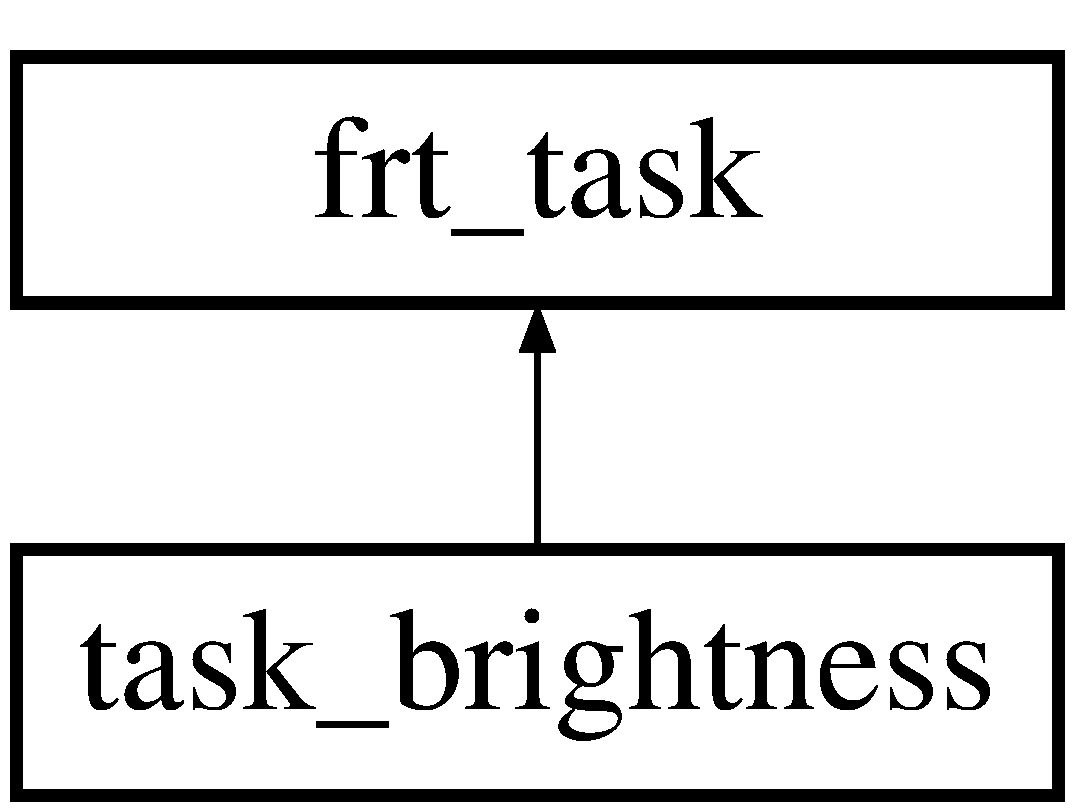
\includegraphics[height=2.000000cm]{classtask__brightness}
\end{center}
\end{figure}
\subsection*{Public Member Functions}
\begin{DoxyCompactItemize}
\item 
\hyperlink{classtask__brightness_a5802baf3a0c9fe53ccbce8966d1fad47}{task\+\_\+brightness} (const char $\ast$, unsigned port\+B\+A\+S\+E\+\_\+\+T\+Y\+P\+E, size\+\_\+t, emstream $\ast$)
\item 
void \hyperlink{classtask__brightness_a615beac07a99f0856f048a46fd9a3898}{run} (void)
\end{DoxyCompactItemize}


\subsection{Detailed Description}
This task controls the brightness of an L\+E\+D using an analog input from the A/\+D converter. 

The A/\+D converter is run using a driver in files {\ttfamily \hyperlink{adc_8h}{adc.\+h}} and {\ttfamily \hyperlink{adc_8cpp}{adc.\+cpp}}. Code in this task sets up a timer/counter in P\+W\+M mode and controls the L\+E\+D's average brightness. 

Definition at line 60 of file task\+\_\+brightness.\+h.



\subsection{Constructor \& Destructor Documentation}
\hypertarget{classtask__brightness_a5802baf3a0c9fe53ccbce8966d1fad47}{\index{task\+\_\+brightness@{task\+\_\+brightness}!task\+\_\+brightness@{task\+\_\+brightness}}
\index{task\+\_\+brightness@{task\+\_\+brightness}!task\+\_\+brightness@{task\+\_\+brightness}}
\subsubsection[{task\+\_\+brightness}]{\setlength{\rightskip}{0pt plus 5cm}task\+\_\+brightness\+::task\+\_\+brightness (
\begin{DoxyParamCaption}
\item[{const char $\ast$}]{a\+\_\+name, }
\item[{unsigned port\+B\+A\+S\+E\+\_\+\+T\+Y\+P\+E}]{a\+\_\+priority, }
\item[{size\+\_\+t}]{a\+\_\+stack\+\_\+size, }
\item[{emstream $\ast$}]{p\+\_\+ser\+\_\+dev}
\end{DoxyParamCaption}
)}}\label{classtask__brightness_a5802baf3a0c9fe53ccbce8966d1fad47}
This constructor creates a task which controls the brightness of an L\+E\+D using input from an A/\+D converter. The main job of this constructor is to call the constructor of parent class ({\ttfamily frt\+\_\+task} ); the parent's constructor the work. 
\begin{DoxyParams}{Parameters}
{\em a\+\_\+name} & A character string which will be the name of this task \\
\hline
{\em a\+\_\+priority} & The priority at which this task will initially run (default\+: 0) \\
\hline
{\em a\+\_\+stack\+\_\+size} & The size of this task's stack in bytes (default\+: config\+M\+I\+N\+I\+M\+A\+L\+\_\+\+S\+T\+A\+C\+K\+\_\+\+S\+I\+Z\+E) \\
\hline
{\em p\+\_\+ser\+\_\+dev} & Pointer to a serial device (port, radio, S\+D card, etc.) which can be used by this task to communicate (default\+: N\+U\+L\+L) \\
\hline
\end{DoxyParams}


Definition at line 49 of file task\+\_\+brightness.\+cpp.



\subsection{Member Function Documentation}
\hypertarget{classtask__brightness_a615beac07a99f0856f048a46fd9a3898}{\index{task\+\_\+brightness@{task\+\_\+brightness}!run@{run}}
\index{run@{run}!task\+\_\+brightness@{task\+\_\+brightness}}
\subsubsection[{run}]{\setlength{\rightskip}{0pt plus 5cm}void task\+\_\+brightness\+::run (
\begin{DoxyParamCaption}
\item[{void}]{}
\end{DoxyParamCaption}
)}}\label{classtask__brightness_a615beac07a99f0856f048a46fd9a3898}
This method is called once by the R\+T\+O\+S scheduler. Each time around the for (;;) loop, it reads the A/\+D converter and uses the result to control the brightness of an L\+E\+D. 

Definition at line 67 of file task\+\_\+brightness.\+cpp.



References adc\+::read\+\_\+oversampled().



The documentation for this class was generated from the following files\+:\begin{DoxyCompactItemize}
\item 
\hyperlink{task__brightness_8h}{task\+\_\+brightness.\+h}\item 
\hyperlink{task__brightness_8cpp}{task\+\_\+brightness.\+cpp}\end{DoxyCompactItemize}

\hypertarget{classtask__user}{\section{task\+\_\+user Class Reference}
\label{classtask__user}\index{task\+\_\+user@{task\+\_\+user}}
}


{\ttfamily \#include $<$task\+\_\+user.\+h$>$}

Inheritance diagram for task\+\_\+user\+:\begin{figure}[H]
\begin{center}
\leavevmode
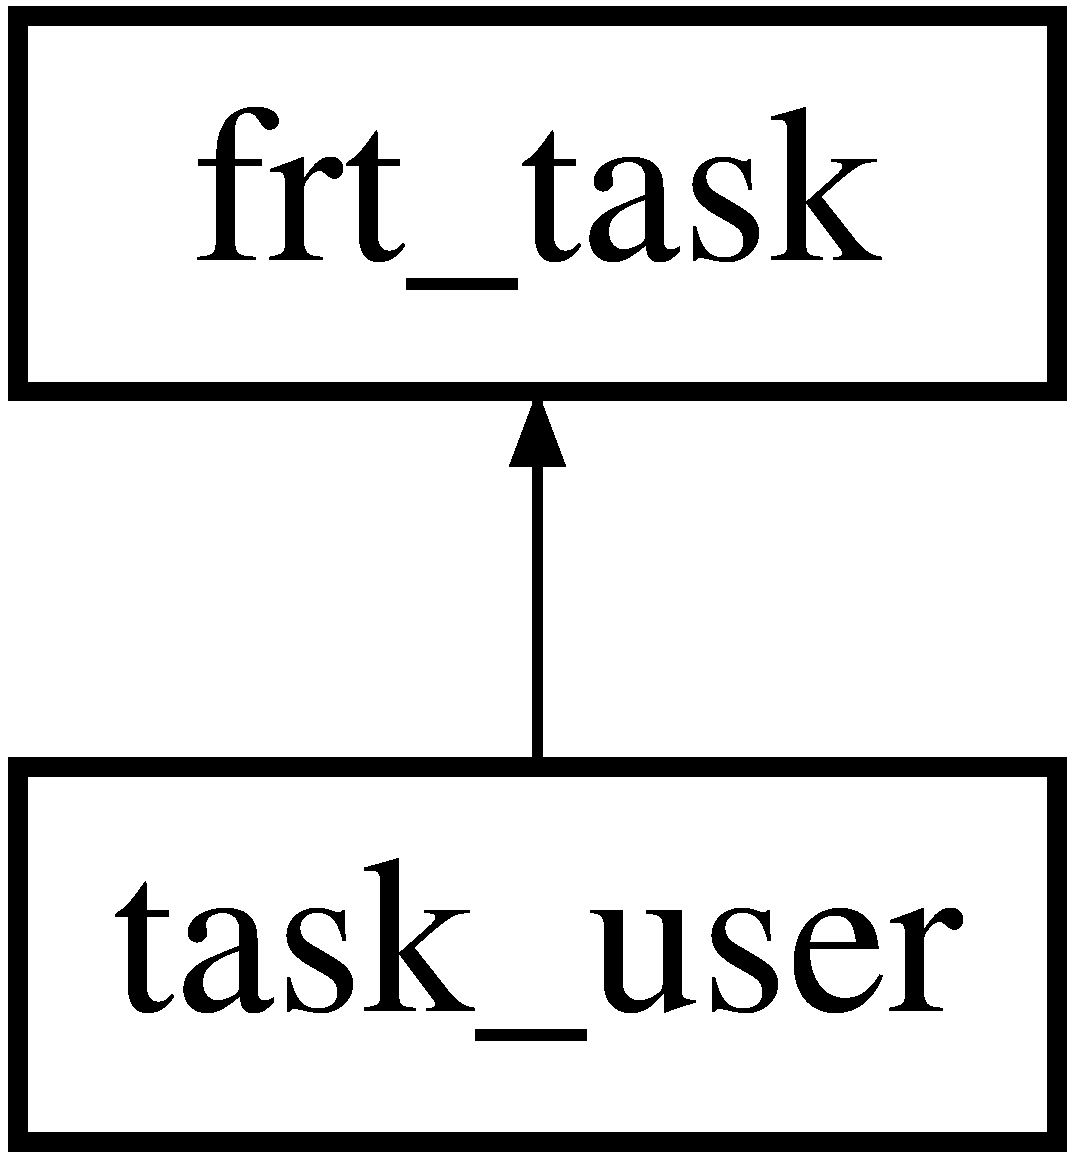
\includegraphics[height=2.000000cm]{classtask__user}
\end{center}
\end{figure}
\subsection*{Public Member Functions}
\begin{DoxyCompactItemize}
\item 
\hyperlink{classtask__user_a3aba77563b375bb14838800608da48bc}{task\+\_\+user} (const char $\ast$, unsigned port\+B\+A\+S\+E\+\_\+\+T\+Y\+P\+E, size\+\_\+t, emstream $\ast$)
\item 
void \hyperlink{classtask__user_adca6429d57be25e8d411414fc8ad75af}{run} (void)
\end{DoxyCompactItemize}
\subsection*{Protected Member Functions}
\begin{DoxyCompactItemize}
\item 
void \hyperlink{classtask__user_a75475060f83bae1e44bcc8a5c34015c7}{print\+\_\+help\+\_\+message} (void)
\item 
void \hyperlink{classtask__user_a105bebbd9cb1031154c3dfc3662db4a0}{show\+\_\+status} (void)
\end{DoxyCompactItemize}


\subsection{Detailed Description}
This task interacts with the user for force him/her to do what he/she is told. What a rude task this is. Then again, computers tend to be that way; if they're polite with you, they're probably spying on you. 

Definition at line 59 of file task\+\_\+user.\+h.



\subsection{Constructor \& Destructor Documentation}
\hypertarget{classtask__user_a3aba77563b375bb14838800608da48bc}{\index{task\+\_\+user@{task\+\_\+user}!task\+\_\+user@{task\+\_\+user}}
\index{task\+\_\+user@{task\+\_\+user}!task\+\_\+user@{task\+\_\+user}}
\subsubsection[{task\+\_\+user}]{\setlength{\rightskip}{0pt plus 5cm}task\+\_\+user\+::task\+\_\+user (
\begin{DoxyParamCaption}
\item[{const char $\ast$}]{a\+\_\+name, }
\item[{unsigned port\+B\+A\+S\+E\+\_\+\+T\+Y\+P\+E}]{a\+\_\+priority, }
\item[{size\+\_\+t}]{a\+\_\+stack\+\_\+size, }
\item[{emstream $\ast$}]{p\+\_\+ser\+\_\+dev}
\end{DoxyParamCaption}
)}}\label{classtask__user_a3aba77563b375bb14838800608da48bc}
This constructor creates a new data acquisition task. Its main job is to call the parent class's constructor which does most of the work. 
\begin{DoxyParams}{Parameters}
{\em a\+\_\+name} & A character string which will be the name of this task \\
\hline
{\em a\+\_\+priority} & The priority at which this task will initially run (default\+: 0) \\
\hline
{\em a\+\_\+stack\+\_\+size} & The size of this task's stack in bytes (default\+: config\+M\+I\+N\+I\+M\+A\+L\+\_\+\+S\+T\+A\+C\+K\+\_\+\+S\+I\+Z\+E) \\
\hline
{\em p\+\_\+ser\+\_\+dev} & Pointer to a serial device (port, radio, S\+D card, etc.) which can be used by this task to communicate (default\+: N\+U\+L\+L) \\
\hline
\end{DoxyParams}


Definition at line 53 of file task\+\_\+user.\+cpp.



\subsection{Member Function Documentation}
\hypertarget{classtask__user_a75475060f83bae1e44bcc8a5c34015c7}{\index{task\+\_\+user@{task\+\_\+user}!print\+\_\+help\+\_\+message@{print\+\_\+help\+\_\+message}}
\index{print\+\_\+help\+\_\+message@{print\+\_\+help\+\_\+message}!task\+\_\+user@{task\+\_\+user}}
\subsubsection[{print\+\_\+help\+\_\+message}]{\setlength{\rightskip}{0pt plus 5cm}void task\+\_\+user\+::print\+\_\+help\+\_\+message (
\begin{DoxyParamCaption}
\item[{void}]{}
\end{DoxyParamCaption}
)\hspace{0.3cm}{\ttfamily [protected]}}}\label{classtask__user_a75475060f83bae1e44bcc8a5c34015c7}
This method prints a simple help message. 

Definition at line 202 of file task\+\_\+user.\+cpp.



References P\+R\+O\+G\+R\+A\+M\+\_\+\+V\+E\+R\+S\+I\+O\+N.



Referenced by run().

\hypertarget{classtask__user_adca6429d57be25e8d411414fc8ad75af}{\index{task\+\_\+user@{task\+\_\+user}!run@{run}}
\index{run@{run}!task\+\_\+user@{task\+\_\+user}}
\subsubsection[{run}]{\setlength{\rightskip}{0pt plus 5cm}void task\+\_\+user\+::run (
\begin{DoxyParamCaption}
\item[{void}]{}
\end{DoxyParamCaption}
)}}\label{classtask__user_adca6429d57be25e8d411414fc8ad75af}
This method is called by the R\+T\+O\+S once to run the task loop for ever and ever.

This task interacts with the user for force him/her to do what he/she is told. It is just following the modern government model of \char`\"{}\+This is the land of the free...
free to do exactly what you're told.\char`\"{} 

Definition at line 71 of file task\+\_\+user.\+cpp.



References print\+\_\+help\+\_\+message(), print\+\_\+ser\+\_\+queue, and show\+\_\+status().

\hypertarget{classtask__user_a105bebbd9cb1031154c3dfc3662db4a0}{\index{task\+\_\+user@{task\+\_\+user}!show\+\_\+status@{show\+\_\+status}}
\index{show\+\_\+status@{show\+\_\+status}!task\+\_\+user@{task\+\_\+user}}
\subsubsection[{show\+\_\+status}]{\setlength{\rightskip}{0pt plus 5cm}void task\+\_\+user\+::show\+\_\+status (
\begin{DoxyParamCaption}
\item[{void}]{}
\end{DoxyParamCaption}
)\hspace{0.3cm}{\ttfamily [protected]}}}\label{classtask__user_a105bebbd9cb1031154c3dfc3662db4a0}
This method displays information about the status of the system, including the following\+: \begin{DoxyItemize}
\item The name and version of the program \item The name, status, priority, and free stack space of each task \item Processor cycles used by each task \item Amount of heap space free and setting of R\+T\+O\+S tick timer \end{DoxyItemize}


Definition at line 225 of file task\+\_\+user.\+cpp.



References P\+R\+O\+G\+R\+A\+M\+\_\+\+V\+E\+R\+S\+I\+O\+N.



Referenced by run().



The documentation for this class was generated from the following files\+:\begin{DoxyCompactItemize}
\item 
\hyperlink{task__user_8h}{task\+\_\+user.\+h}\item 
\hyperlink{task__user_8cpp}{task\+\_\+user.\+cpp}\end{DoxyCompactItemize}

\chapter{File Documentation}
\hypertarget{adc_8cpp}{\section{adc.\+cpp File Reference}
\label{adc_8cpp}\index{adc.\+cpp@{adc.\+cpp}}
}
{\ttfamily \#include $<$stdlib.\+h$>$}\\*
{\ttfamily \#include $<$avr/io.\+h$>$}\\*
{\ttfamily \#include \char`\"{}rs232int.\+h\char`\"{}}\\*
{\ttfamily \#include \char`\"{}adc.\+h\char`\"{}}\\*
\subsection*{Functions}
\begin{DoxyCompactItemize}
\item 
emstream \& \hyperlink{adc_8cpp_afb33ca9fe94765ee57079e7feb03f975}{operator$<$$<$} (emstream \&serpt, \hyperlink{classadc}{adc} \&a2d)
\begin{DoxyCompactList}\small\item\em This overloaded operator \char`\"{}prints\char`\"{} the A/\+D converter. \end{DoxyCompactList}\end{DoxyCompactItemize}


\subsection{Detailed Description}
This file contains a very simple A/\+D converter driver. This driver should be

Revisions\+: \begin{DoxyItemize}
\item 01-\/15-\/2008 J\+R\+R Original (somewhat useful) file \item 10-\/11-\/2012 J\+R\+R Less original, more useful file with Free\+R\+T\+O\+S mutex added \item 10-\/12-\/2012 J\+R\+R There was a bug in the mutex code, and it has been fixed\end{DoxyItemize}
License\+: This file is copyright 2012 by J\+R Ridgely and released under the Lesser G\+N\+U Public License, version 2. It intended for educational use only, but its use is not limited thereto. 

Definition in file \hyperlink{adc_8cpp_source}{adc.\+cpp}.



\subsection{Function Documentation}
\hypertarget{adc_8cpp_afb33ca9fe94765ee57079e7feb03f975}{\index{adc.\+cpp@{adc.\+cpp}!operator$<$$<$@{operator$<$$<$}}
\index{operator$<$$<$@{operator$<$$<$}!adc.\+cpp@{adc.\+cpp}}
\subsubsection[{operator$<$$<$}]{\setlength{\rightskip}{0pt plus 5cm}emstream\& operator$<$$<$ (
\begin{DoxyParamCaption}
\item[{emstream \&}]{serpt, }
\item[{{\bf adc} \&}]{a2d}
\end{DoxyParamCaption}
)}}\label{adc_8cpp_afb33ca9fe94765ee57079e7feb03f975}


This overloaded operator \char`\"{}prints\char`\"{} the A/\+D converter. 

{\bfseries Details\+:} This overloaded operator will return A\+D\+M\+U\+X and A\+D\+C\+S\+R\+A in binary. 
\begin{DoxyParams}{Parameters}
{\em serpt} & The serial port where the printout will be printed. \\
\hline
{\em a2d} & The A/\+D driver which is being printed. \\
\hline
\end{DoxyParams}
\begin{DoxyReturn}{Returns}
A reference to the same serial device that the information is written to. This is used to string together things to write with \char`\"{}$<$$<$\char`\"{} operators 
\end{DoxyReturn}


Definition at line 117 of file adc.\+cpp.


\hypertarget{adc_8h}{\section{adc.\-h \-File \-Reference}
\label{adc_8h}\index{adc.\-h@{adc.\-h}}
}
{\ttfamily \#include \char`\"{}emstream.\-h\char`\"{}}\*
{\ttfamily \#include \char`\"{}\-Free\-R\-T\-O\-S.\-h\char`\"{}}\*
{\ttfamily \#include \char`\"{}task.\-h\char`\"{}}\*
{\ttfamily \#include \char`\"{}queue.\-h\char`\"{}}\*
{\ttfamily \#include \char`\"{}semphr.\-h\char`\"{}}\*
\subsection*{\-Classes}
\begin{DoxyCompactItemize}
\item 
class \hyperlink{classadc}{adc}
\begin{DoxyCompactList}\small\item\em \-This class should run the \-A/\-D converter on an \-A\-V\-R processor. \end{DoxyCompactList}\end{DoxyCompactItemize}
\subsection*{\-Functions}
\begin{DoxyCompactItemize}
\item 
emstream \& \hyperlink{adc_8h_a6e6d1e227b216fe2a1fee9b0ea52180d}{operator$<$$<$} (emstream \&, \hyperlink{classadc}{adc} \&)
\begin{DoxyCompactList}\small\item\em \-This overloaded operator \char`\"{}prints\char`\"{} the \-A/\-D converter. \end{DoxyCompactList}\end{DoxyCompactItemize}


\subsection{\-Detailed \-Description}
\-This file contains a very simple \-A/\-D converter driver. \-The driver is hopefully thread safe in \-Free\-R\-T\-O\-S due to the use of a mutex to prevent its use by multiple tasks at the same time. \-There is no protection from priority inversion, however, except for the priority elevation in the mutex.

\-Revisions\-: \begin{DoxyItemize}
\item 01-\/15-\/2008 \-J\-R\-R \-Original (somewhat useful) file \item 10-\/11-\/2012 \-J\-R\-R \-Less original, more useful file with \-Free\-R\-T\-O\-S mutex added \item 10-\/12-\/2012 \-J\-R\-R \-There was a bug in the mutex code, and it has been fixed\end{DoxyItemize}
\-License\-: \-This file is copyright 2012 by \-J\-R \-Ridgely and released under the \-Lesser \-G\-N\-U \-Public \-License, version 2. \-It intended for educational use only, but its use is not limited thereto. 

\-Definition in file \hyperlink{adc_8h_source}{adc.\-h}.



\subsection{\-Function \-Documentation}
\hypertarget{adc_8h_a6e6d1e227b216fe2a1fee9b0ea52180d}{\index{adc.\-h@{adc.\-h}!operator$<$$<$@{operator$<$$<$}}
\index{operator$<$$<$@{operator$<$$<$}!adc.h@{adc.\-h}}
\subsubsection[{operator$<$$<$}]{\setlength{\rightskip}{0pt plus 5cm}emstream\& operator$<$$<$ (
\begin{DoxyParamCaption}
\item[{emstream \&}]{serpt, }
\item[{{\bf adc} \&}]{a2d}
\end{DoxyParamCaption}
)}}\label{adc_8h_a6e6d1e227b216fe2a1fee9b0ea52180d}


\-This overloaded operator \char`\"{}prints\char`\"{} the \-A/\-D converter. 

{\bfseries \-Details\-:} \-This overloaded operator will return \-A\-D\-M\-U\-X and \-A\-D\-C\-S\-R\-A in binary. 
\begin{DoxyParams}{\-Parameters}
{\em serpt} & \-The serial port where the printout will be printed. \\
\hline
{\em a2d} & \-The \-A/\-D driver which is being printed. \\
\hline
\end{DoxyParams}
\begin{DoxyReturn}{\-Returns}
\-A reference to the same serial device that the information is written to. \-This is used to string together things to write with \char`\"{}$<$$<$\char`\"{} operators 
\end{DoxyReturn}


\-Definition at line 117 of file adc.\-cpp.


\hypertarget{lab1__main_8cpp}{\section{lab1\+\_\+main.\+cpp File Reference}
\label{lab1__main_8cpp}\index{lab1\+\_\+main.\+cpp@{lab1\+\_\+main.\+cpp}}
}
{\ttfamily \#include $<$stdlib.\+h$>$}\\*
{\ttfamily \#include $<$avr/io.\+h$>$}\\*
{\ttfamily \#include $<$avr/wdt.\+h$>$}\\*
{\ttfamily \#include $<$string.\+h$>$}\\*
{\ttfamily \#include \char`\"{}Free\+R\+T\+O\+S.\+h\char`\"{}}\\*
{\ttfamily \#include \char`\"{}task.\+h\char`\"{}}\\*
{\ttfamily \#include \char`\"{}queue.\+h\char`\"{}}\\*
{\ttfamily \#include \char`\"{}croutine.\+h\char`\"{}}\\*
{\ttfamily \#include \char`\"{}rs232int.\+h\char`\"{}}\\*
{\ttfamily \#include \char`\"{}time\+\_\+stamp.\+h\char`\"{}}\\*
{\ttfamily \#include \char`\"{}frt\+\_\+task.\+h\char`\"{}}\\*
{\ttfamily \#include \char`\"{}frt\+\_\+text\+\_\+queue.\+h\char`\"{}}\\*
{\ttfamily \#include \char`\"{}frt\+\_\+queue.\+h\char`\"{}}\\*
{\ttfamily \#include \char`\"{}frt\+\_\+shared\+\_\+data.\+h\char`\"{}}\\*
{\ttfamily \#include \char`\"{}shares.\+h\char`\"{}}\\*
{\ttfamily \#include \char`\"{}task\+\_\+brightness.\+h\char`\"{}}\\*
{\ttfamily \#include \char`\"{}task\+\_\+user.\+h\char`\"{}}\\*
\subsection*{Functions}
\begin{DoxyCompactItemize}
\item 
frt\+\_\+text\+\_\+queue \hyperlink{lab1__main_8cpp_a4c623cb3c8a60e67138367480c1ee0d2}{print\+\_\+ser\+\_\+queue} (32, N\+U\+L\+L, 10)
\item 
int \hyperlink{lab1__main_8cpp_a840291bc02cba5474a4cb46a9b9566fe}{main} (void)
\end{DoxyCompactItemize}


\subsection{Detailed Description}
This file contains the \hyperlink{lab1__main_8cpp_a840291bc02cba5474a4cb46a9b9566fe}{main()} code for a program which runs the M\+E405 board for M\+E405 lab 1. This program currently uses obfuscated code to use an A/\+D converter to convert an analog signal into an L\+E\+D brightness via pulse width modulation. {\bfseries This} {\bfseries comment} {\bfseries is} {\bfseries quite} {\bfseries messed} {\bfseries up} {\bfseries and} {\bfseries the} {\bfseries student} {\bfseries should} {\bfseries fix} {\bfseries it} {\bfseries so} {\bfseries that} {\bfseries it} {\bfseries accurately} {\bfseries reflects} {\bfseries the} {\bfseries function} {\bfseries of} {\bfseries the} {\bfseries program} {\bfseries which} {\bfseries is} {\bfseries handed} {\bfseries in} {\bfseries for} {\bfseries this} {\bfseries assignment}.

Revisions\+: \begin{DoxyItemize}
\item 09-\/30-\/2012 J\+R\+R Original file was a one-\/file demonstration with two tasks \item 10-\/05-\/2012 J\+R\+R Split into multiple files, one for each task plus a main one \item 10-\/30-\/2012 J\+R\+R A hopefully somewhat stable version with global queue pointers and the new operator used for most memory allocation \item 11-\/04-\/2012 J\+R\+R Free\+R\+T\+O\+S Swoop demo program changed to a sweet test suite \item 01-\/05-\/2012 J\+R\+R Program reconfigured as M\+E405 Lab 1 starting point \item 03-\/28-\/2014 J\+R\+R Pointers to shared variables and queues changed to references\end{DoxyItemize}
License\+: This file is copyright 2012 by J\+R Ridgely and released under the Lesser G\+N\+U Public License, version 2. It intended for educational use only, but its use is not limited thereto. 

Definition in file \hyperlink{lab1__main_8cpp_source}{lab1\+\_\+main.\+cpp}.



\subsection{Function Documentation}
\hypertarget{lab1__main_8cpp_a840291bc02cba5474a4cb46a9b9566fe}{\index{lab1\+\_\+main.\+cpp@{lab1\+\_\+main.\+cpp}!main@{main}}
\index{main@{main}!lab1\+\_\+main.\+cpp@{lab1\+\_\+main.\+cpp}}
\subsubsection[{main}]{\setlength{\rightskip}{0pt plus 5cm}int main (
\begin{DoxyParamCaption}
\item[{void}]{}
\end{DoxyParamCaption}
)}}\label{lab1__main_8cpp_a840291bc02cba5474a4cb46a9b9566fe}
The main function sets up the R\+T\+O\+S. Some test tasks are created. Then the scheduler is started up; the scheduler runs until power is turned off or there's a reset. \begin{DoxyReturn}{Returns}
This is a real-\/time microcontroller program which doesn't return. Ever. 
\end{DoxyReturn}


Definition at line 80 of file lab1\+\_\+main.\+cpp.

\hypertarget{lab1__main_8cpp_a4c623cb3c8a60e67138367480c1ee0d2}{\index{lab1\+\_\+main.\+cpp@{lab1\+\_\+main.\+cpp}!print\+\_\+ser\+\_\+queue@{print\+\_\+ser\+\_\+queue}}
\index{print\+\_\+ser\+\_\+queue@{print\+\_\+ser\+\_\+queue}!lab1\+\_\+main.\+cpp@{lab1\+\_\+main.\+cpp}}
\subsubsection[{print\+\_\+ser\+\_\+queue}]{\setlength{\rightskip}{0pt plus 5cm}frt\+\_\+text\+\_\+queue print\+\_\+ser\+\_\+queue (
\begin{DoxyParamCaption}
\item[{32}]{, }
\item[{N\+U\+L\+L}]{, }
\item[{10}]{}
\end{DoxyParamCaption}
)}}\label{lab1__main_8cpp_a4c623cb3c8a60e67138367480c1ee0d2}
This is a print queue, descended from {\ttfamily emstream} so that things can be printed into the queue using the \char`\"{}$<$$<$\char`\"{} operator and they'll come out the other end as a stream of characters. It's used by tasks that send things to the user interface task to be printed. 
\hypertarget{shares_8h}{\section{shares.\+h File Reference}
\label{shares_8h}\index{shares.\+h@{shares.\+h}}
}
\subsection*{Variables}
\begin{DoxyCompactItemize}
\item 
\hypertarget{shares_8h_aa7d8f7a1c41bee143392fe322e8a07b2}{frt\+\_\+text\+\_\+queue \hyperlink{shares_8h_aa7d8f7a1c41bee143392fe322e8a07b2}{print\+\_\+ser\+\_\+queue}}\label{shares_8h_aa7d8f7a1c41bee143392fe322e8a07b2}

\begin{DoxyCompactList}\small\item\em This queue allows tasks to send characters to the user interface task for display. \end{DoxyCompactList}\end{DoxyCompactItemize}


\subsection{Detailed Description}
This file contains extern declarations for queues and other inter-\/task data communication objects used in a M\+E405/507/\+Free\+R\+T\+O\+S project.

Revisions\+: \begin{DoxyItemize}
\item 09-\/30-\/2012 J\+R\+R Original file was a one-\/file demonstration with two tasks \item 10-\/05-\/2012 J\+R\+R Split into multiple files, one for each task plus a main one \item 10-\/29-\/2012 J\+R\+R Reorganized with global queue and shared data references\end{DoxyItemize}
License\+: This file is copyright 2012 by J\+R Ridgely and released under the Lesser G\+N\+U Public License, version 2. It intended for educational use only, but its use is not limited thereto. 

Definition in file \hyperlink{shares_8h_source}{shares.\+h}.


\hypertarget{task__brightness_8cpp}{\section{task\+\_\+brightness.\+cpp File Reference}
\label{task__brightness_8cpp}\index{task\+\_\+brightness.\+cpp@{task\+\_\+brightness.\+cpp}}
}
{\ttfamily \#include \char`\"{}frt\+\_\+text\+\_\+queue.\+h\char`\"{}}\\*
{\ttfamily \#include \char`\"{}task\+\_\+brightness.\+h\char`\"{}}\\*
{\ttfamily \#include \char`\"{}shares.\+h\char`\"{}}\\*


\subsection{Detailed Description}
This file contains the code for a task class which controls the brightness of an L\+E\+D using a voltage measured from the A/\+D as input. The fun part\+: the brightness that is being controlled can be on another A\+V\+R computer, with signals being sent and received via wireless transceivers.

Revisions\+: \begin{DoxyItemize}
\item 09-\/30-\/2012 J\+R\+R Original file was a one-\/file demonstration with two tasks \item 10-\/05-\/2012 J\+R\+R Split into multiple files, one for each task \item 10-\/25-\/2012 J\+R\+R Changed to a more fully C++ version with class task\+\_\+sender \item 10-\/27-\/2012 J\+R\+R Altered from data sending task into L\+E\+D blinking class \item 11-\/04-\/2012 J\+R\+R Altered again into the multi-\/task monstrosity \item 12-\/13-\/2012 J\+R\+R Yet again transmogrified; now it controls L\+E\+D brightness\end{DoxyItemize}
License\+: This file is copyright 2012 by J\+R Ridgely and released under the Lesser G\+N\+U Public License, version 2. It intended for educational use only, but its use is not limited thereto. 

Definition in file \hyperlink{task__brightness_8cpp_source}{task\+\_\+brightness.\+cpp}.


\hypertarget{task__brightness_8h}{\section{task\+\_\+brightness.\+h File Reference}
\label{task__brightness_8h}\index{task\+\_\+brightness.\+h@{task\+\_\+brightness.\+h}}
}
{\ttfamily \#include $<$stdlib.\+h$>$}\\*
{\ttfamily \#include $<$avr/io.\+h$>$}\\*
{\ttfamily \#include \char`\"{}Free\+R\+T\+O\+S.\+h\char`\"{}}\\*
{\ttfamily \#include \char`\"{}task.\+h\char`\"{}}\\*
{\ttfamily \#include \char`\"{}queue.\+h\char`\"{}}\\*
{\ttfamily \#include \char`\"{}frt\+\_\+task.\+h\char`\"{}}\\*
{\ttfamily \#include \char`\"{}time\+\_\+stamp.\+h\char`\"{}}\\*
{\ttfamily \#include \char`\"{}frt\+\_\+queue.\+h\char`\"{}}\\*
{\ttfamily \#include \char`\"{}frt\+\_\+shared\+\_\+data.\+h\char`\"{}}\\*
{\ttfamily \#include \char`\"{}rs232int.\+h\char`\"{}}\\*
{\ttfamily \#include \char`\"{}adc.\+h\char`\"{}}\\*
\subsection*{Classes}
\begin{DoxyCompactItemize}
\item 
class \hyperlink{classtask__brightness}{task\+\_\+brightness}
\begin{DoxyCompactList}\small\item\em This task controls the brightness of an L\+E\+D using an analog input from the A/\+D converter. \end{DoxyCompactList}\end{DoxyCompactItemize}


\subsection{Detailed Description}
This file contains the header for a task class that controls the brightness of an L\+E\+D using a voltage measured from the A/\+D as input. The fun part\+: the brightness that is being controlled can be on another A\+V\+R computer, with signals being sent and received via wireless transceivers.

Revisions\+: \begin{DoxyItemize}
\item 09-\/30-\/2012 J\+R\+R Original file was a one-\/file demonstration with two tasks \item 10-\/05-\/2012 J\+R\+R Split into multiple files, one for each task \item 10-\/25-\/2012 J\+R\+R Changed to a more fully C++ version with class task\+\_\+sender \item 10-\/27-\/2012 J\+R\+R Altered from data sending task into L\+E\+D blinking class \item 11-\/04-\/2012 J\+R\+R Altered again into the multi-\/task monstrosity \item 12-\/13-\/2012 J\+R\+R Yet again transmogrified; now it controls L\+E\+D brightness\end{DoxyItemize}
License\+: This file is copyright 2012 by J\+R Ridgely and released under the Lesser G\+N\+U Public License, version 2. It intended for educational use only, but its use is not limited thereto. 

Definition in file \hyperlink{task__brightness_8h_source}{task\+\_\+brightness.\+h}.


\hypertarget{task__user_8cpp}{\section{task\+\_\+user.\+cpp File Reference}
\label{task__user_8cpp}\index{task\+\_\+user.\+cpp@{task\+\_\+user.\+cpp}}
}
{\ttfamily \#include $<$avr/io.\+h$>$}\\*
{\ttfamily \#include $<$avr/wdt.\+h$>$}\\*
{\ttfamily \#include \char`\"{}shared\+\_\+data\+\_\+sender.\+h\char`\"{}}\\*
{\ttfamily \#include \char`\"{}shared\+\_\+data\+\_\+receiver.\+h\char`\"{}}\\*
{\ttfamily \#include \char`\"{}task\+\_\+user.\+h\char`\"{}}\\*
\subsection*{Variables}
\begin{DoxyCompactItemize}
\item 
const port\+Tick\+Type \hyperlink{task__user_8cpp_a80f7a5c45b5679c45dd218506ab058f0}{ticks\+\_\+to\+\_\+delay} = ((config\+T\+I\+C\+K\+\_\+\+R\+A\+T\+E\+\_\+\+H\+Z / 1000) $\ast$ 5)
\end{DoxyCompactItemize}


\subsection{Detailed Description}
This file contains source code for a user interface task for a M\+E405/\+Free\+R\+T\+O\+S test suite.

Revisions\+: \begin{DoxyItemize}
\item 09-\/30-\/2012 J\+R\+R Original file was a one-\/file demonstration with two tasks \item 10-\/05-\/2012 J\+R\+R Split into multiple files, one for each task \item 10-\/25-\/2012 J\+R\+R Changed to a more fully C++ version with class \hyperlink{classtask__user}{task\+\_\+user} \item 11-\/04-\/2012 J\+R\+R Modified from the data acquisition example to the test suite\end{DoxyItemize}
License\+: This file is copyright 2012 by J\+R Ridgely and released under the Lesser G\+N\+U Public License, version 2. It intended for educational use only, but its use is not limited thereto. 

Definition in file \hyperlink{task__user_8cpp_source}{task\+\_\+user.\+cpp}.



\subsection{Variable Documentation}
\hypertarget{task__user_8cpp_a80f7a5c45b5679c45dd218506ab058f0}{\index{task\+\_\+user.\+cpp@{task\+\_\+user.\+cpp}!ticks\+\_\+to\+\_\+delay@{ticks\+\_\+to\+\_\+delay}}
\index{ticks\+\_\+to\+\_\+delay@{ticks\+\_\+to\+\_\+delay}!task\+\_\+user.\+cpp@{task\+\_\+user.\+cpp}}
\subsubsection[{ticks\+\_\+to\+\_\+delay}]{\setlength{\rightskip}{0pt plus 5cm}const port\+Tick\+Type ticks\+\_\+to\+\_\+delay = ((config\+T\+I\+C\+K\+\_\+\+R\+A\+T\+E\+\_\+\+H\+Z / 1000) $\ast$ 5)}}\label{task__user_8cpp_a80f7a5c45b5679c45dd218506ab058f0}
This constant sets how many R\+T\+O\+S ticks the task delays if the user's not talking. The duration is calculated to be about 5 ms. 

Definition at line 39 of file task\+\_\+user.\+cpp.


\hypertarget{task__user_8h}{\section{task\+\_\+user.\+h File Reference}
\label{task__user_8h}\index{task\+\_\+user.\+h@{task\+\_\+user.\+h}}
}
{\ttfamily \#include $<$stdlib.\+h$>$}\\*
{\ttfamily \#include \char`\"{}Free\+R\+T\+O\+S.\+h\char`\"{}}\\*
{\ttfamily \#include \char`\"{}task.\+h\char`\"{}}\\*
{\ttfamily \#include \char`\"{}queue.\+h\char`\"{}}\\*
{\ttfamily \#include \char`\"{}rs232int.\+h\char`\"{}}\\*
{\ttfamily \#include \char`\"{}adc.\+h\char`\"{}}\\*
{\ttfamily \#include \char`\"{}time\+\_\+stamp.\+h\char`\"{}}\\*
{\ttfamily \#include \char`\"{}frt\+\_\+task.\+h\char`\"{}}\\*
{\ttfamily \#include \char`\"{}frt\+\_\+queue.\+h\char`\"{}}\\*
{\ttfamily \#include \char`\"{}frt\+\_\+text\+\_\+queue.\+h\char`\"{}}\\*
{\ttfamily \#include \char`\"{}frt\+\_\+shared\+\_\+data.\+h\char`\"{}}\\*
{\ttfamily \#include \char`\"{}shares.\+h\char`\"{}}\\*
\subsection*{Classes}
\begin{DoxyCompactItemize}
\item 
class \hyperlink{classtask__user}{task\+\_\+user}
\end{DoxyCompactItemize}
\subsection*{Macros}
\begin{DoxyCompactItemize}
\item 
\hypertarget{task__user_8h_a2f10abd650e471fae2d7e8c63d41206a}{\#define \hyperlink{task__user_8h_a2f10abd650e471fae2d7e8c63d41206a}{P\+R\+O\+G\+R\+A\+M\+\_\+\+V\+E\+R\+S\+I\+O\+N}~P\+M\+S (\char`\"{}M\+E405 base radio program V0.\+4 \char`\"{})}\label{task__user_8h_a2f10abd650e471fae2d7e8c63d41206a}

\begin{DoxyCompactList}\small\item\em This macro defines a string that identifies the name and version of this program. \end{DoxyCompactList}\end{DoxyCompactItemize}


\subsection{Detailed Description}
This file contains header stuff for a user interface task for a M\+E507/\+Free\+R\+T\+O\+S test suite.

Revisions\+: \begin{DoxyItemize}
\item 09-\/30-\/2012 J\+R\+R Original file was a one-\/file demonstration with two tasks \item 10-\/05-\/2012 J\+R\+R Split into multiple files, one for each task \item 10-\/25-\/2012 J\+R\+R Changed to a more fully C++ version with class \hyperlink{classtask__user}{task\+\_\+user} \item 11-\/04-\/2012 J\+R\+R Modified from the data acquisition example to the test suite\end{DoxyItemize}
License\+: This file is copyright 2012 by J\+R Ridgely and released under the Lesser G\+N\+U Public License, version 2. It intended for educational use only, but its use is not limited thereto. 

Definition in file \hyperlink{task__user_8h_source}{task\+\_\+user.\+h}.


%--- End generated contents ---

% Index
\newpage
\phantomsection
\addcontentsline{toc}{chapter}{Index}
\printindex

\end{document}
